\documentclass[a4paper,11pt]{article}%必须以此为开头,可以在[]内设置栏数,单双面,横竖向
\usepackage[x11names]{xcolor}
\usepackage{ctex}%提供中文支持
\usepackage{graphicx}%用于插入图片
\usepackage{verbatim}%使用\verbatiminput{filename}来直接导入文件中的文本内容
\usepackage{layouts}%用于设置页面布局
\usepackage{makecell}%允许表格的单元格内换行
\usepackage{tikz}
\usetikzlibrary{positioning,shapes.geometric}
%伪代码
\usepackage{algorithm}
\usepackage{algorithmicx}
\usepackage{algpseudocode}
\usepackage{amsmath}
%伪代码
%代码块
\usepackage{ listings}
\definecolor{mygreen}{rgb}{0,0.6,0}
\definecolor{mygray}{rgb}{0.5,0.5,0.5}
\definecolor{mymauve}{rgb}{0.58,0,0.82}
\lstset{ %
	backgroundcolor=\color{white},      % choose the background color
	basicstyle=\footnotesize\ttfamily,  % size of fonts used for the code
	columns=fullflexible,
	tabsize=4,
	breaklines=true,               % automatic line breaking only at whitespace
	captionpos=b,                  % sets the caption-position to bottom
	commentstyle=\color{mygreen},  % comment style
	escapeinside={\%*}{*)},        % if you want to add LaTeX within your code
	keywordstyle=\color{blue},     % keyword style
	stringstyle=\color{mymauve}\ttfamily,  % string literal style
	frame=single,
	rulesepcolor=\color{red!20!green!20!blue!20},
	% identifierstyle=\color{red},
	language=c,
}
%代码块
%跨页伪代码
\makeatletter
\newenvironment{breakablealgorithm}
  {% \begin{breakablealgorithm}
   \begin{center}
     \refstepcounter{algorithm}% New algorithm
     \hrule height.8pt depth0pt \kern2pt% \@fs@pre for \@fs@ruled
     \renewcommand{\caption}[2][\relax]{% Make a new \caption
       {\raggedright\textbf{\ALG@name~\thealgorithm} ##2\par}%
       \ifx\relax##1\relax % #1 is \relax
         \addcontentsline{loa}{algorithm}{\protect\numberline{\thealgorithm}##2}%
       \else % #1 is not \relax
         \addcontentsline{loa}{algorithm}{\protect\numberline{\thealgorithm}##1}%
       \fi
       \kern2pt\hrule\kern2pt
     }
  }{% \end{breakablealgorithm}
     \kern2pt\hrule\relax% \@fs@post for \@fs@ruled
   \end{center}
  }
\makeatother
%跨页伪代码
\newcommand*{\abs}[1]{\lvert #1 \rvert}
\floatname{algorithm}{算法}
\renewcommand{\algorithmicrequire}{\textbf{输入:}}
\renewcommand{\algorithmicensure}{\textbf{输出:}}
\author{姓名: 范潇\phantom{11}学号: 2254298}
\title{欧拉路径 试验报告}
\date{2023年 12月 1日}
\begin{document}
\lstset{breaklines}%这条命令可以让LaTeX自动将长的代码行换行排版
		\lstset{extendedchars=false}%这一条命令可以解决代码跨页时,章节标题,页眉等汉字不显
		%示的问题
		\lstset{numbers=left,numberstyle=\tiny,keywordstyle=\color{blue!70},
			commentstyle=\color{red!50!green!50!blue!50},frame=shadowbox,
			rulesepcolor=\color{red!20!green!20!blue!20},escapeinside=``,
			%xleftmargin=-10em,xrightmargin=-23em,
            aboveskip=1em} 
\pagestyle{plain}%页面风格,plain为中下方有页码.heading是页眉中间有页数,同时有章节名,empty是空页眉页尾
%\thispagestyle{pagestyle}%本页页面风格
% 实验报告格式要求按照模板(使用Markdown等也请保证报告内包含模板中的要素)
% 对字体大小、缩进、颜色等不做强制要求(但尽量代码部分和文字内容有一定区分,可参考vscode配色)
% 实验报告要求在文字简洁的同时将内容表示清楚
% 报告内不要大段贴代码,尽量控制在20页以内
\maketitle
\section{涉及数据结构和相关背景}
\section{实验目的}
\begin{enumerate}
    \item 掌握图的存储结构和基本操作;
    \item 灵活运用图的遍历方法。
\end{enumerate}
\section{实验内容}
编写一个程序,其功能是输出图1中以结点1开始的欧拉路径。

\begin{figure}[htbp]
  \centering
  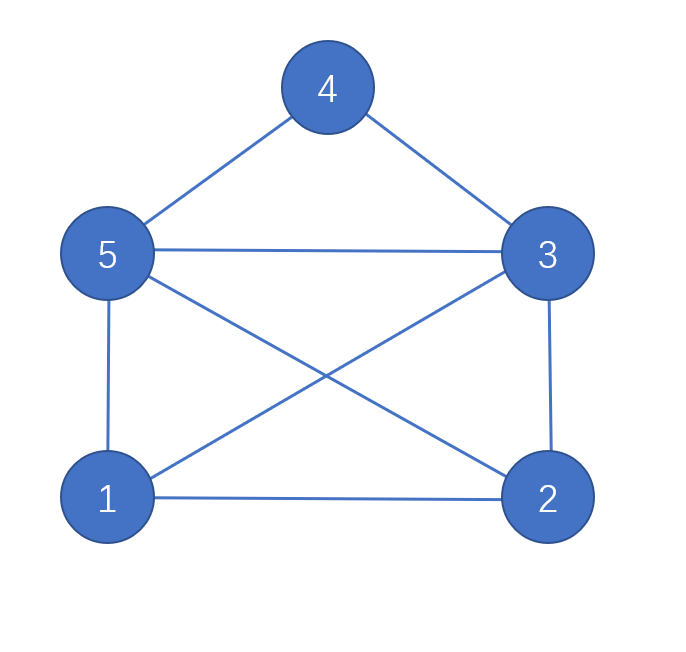
\includegraphics[scale=0.5]{pic.png}
  \caption{map对应的无向图}
\end{figure}
\section{程序实现}
\subsection{数据结构设计}
\begin{lstlisting}[language={[ANSI]C},keywordstyle=\color{blue!70},commentstyle=\color{red!50!green!50!blue!50},frame=shadowbox,
				rulesepcolor=\color{red!20!green!20!blue!20}]
int Map[N][N]={//下标为0的元素为冗余,以确保有效数据的下标从1开始
   {0,0,0,0,0,0},
   {0,0,1,1,0,1},
   {0,1,0,1,0,1},
   {0,1,1,0,1,1},
   {0,0,0,1,0,1},
   {0,1,1,1,1,0}
}; 
\end{lstlisting}
\subsection{功能说明}
\begin{lstlisting}[language={[ANSI]C},keywordstyle=\color{blue!70},commentstyle=\color{red!50!green!50!blue!50},frame=shadowbox,
				rulesepcolor=\color{red!20!green!20!blue!20}]
void DFS(string path,int now)//分别存储当前的路径及其末端结点
{
	if(path.length()==9){//给定图的欧拉路径长度为9
		cout<<path<<endl;
		return;
	}
	for(int i =1;i<N;i++ )	
	  if(Map[now][i]){//对应边存在,且未出现在当前路径中
		  path.push_back(i+'0');//添加进当前路径中
		  Map[now][i]=0;//将对应边置零,表明已经出现在当前路径中
		  Map[i][now]=0;
		  DFS(path,i);//进一步递归
		  path.pop_back();//恢复当前函数调用时的状态
		  Map[now][i]=1;
		  Map[i][now]=1;
	  }
	return ;
}
int main()
{
	DFS("1",1);//从指定结点开始
	return 0;
}
\end{lstlisting}
\subsection{调试分析}
第一次调试时发现输出的序列明显不满足欧拉路径,根据调试模式下的自动变量窗口信息进行排查,发现是因为在第12行结束后只恢复了邻接矩阵,但是并没有恢复
path。
\section{总结与体会}
本题由于要求输出所有的欧拉路径,所以采用循环和递归相结合的形式。在编写程序时,要注意每次循环体开始前,都要保持邻接矩阵和用于存储欧拉路径的变量值不变。
假设所给的无向图有 $e$条边,则其对应的欧拉路径也有 $e$条边,函数需要递归$e+1$层。而在第 $i$层中,至多再次调用$n-i$次自身。因此时间复杂度为
$O(n*e)$,如果使用邻接表实现,则时间复杂度可以降至$O(e^2)$。空间复杂度则是 $O(n^2)$,主要是由邻接矩阵贡献的。
\end{document}